\documentclass[fr]{../../../eplsummary}

\usepackage{../../../eplunits}
\usepackage{../meca-FSAB1202}

% \begin{document}

\hypertitle{M\'ecanique}{2}{FSAB}{1202}
{Mattéo Couplet\and Beno\^it Legat\and Antoine Paris}
{Paul Fisette}

\part{Prérequis mathématiques et notations}
\section{Vecteurs et tenseurs}
Les vecteurs, pour cette synthèse, seront notés $\fv{u}$.
Il y a deux types de vecteurs
\begin{description}
  \item[Lié] L'origine du vecteur est fixée à un certain point.
  \item[Libre] Vecteur sans origine fixe.
\end{description}
La notation $\uv{u}$ indique que $\norm{\uv{u}} = 1$.
$\uv{u}$ est appelé un vecteur unitaire.

\subsection{Base orthonormée}
La base orthonormée $\base{\ui}$ est une base composée de 3 vecteurs unitaires orthogonaux $\ui_1$, $\ui_2$ et $\ui_3$ respectivement arrangés dans l'ordre donné par la règle de la main droite.

Tout vecteur $\fv{u}$ a des coordonnées uniques $u_1, u_2, u_3$ dans $\base{\ui}$.
On a
\[ \fv{u} = u_1\ui_1 + u_2\ui_2 + u_3\ui_3 = \va{\ui}^T u \]
où $\va{\ui} =
\begin{pmatrix}
  \ui_1\\\ui_2\\\ui_3
\end{pmatrix}$ et $u =
\begin{pmatrix}
  u_1 \\ u_2 \\ u_3
\end{pmatrix}$.
Il est important de noter que $\va{\ui}\va{\ui}^T = E$, où $E$ est le tenseur\footnote{Un tenseur
(d'ordre 2) peut être vu comme une application linéaire qui transforme un vecteur \fv{x} en
un autre vecteur $\fv{u}$. N'importe quel tenseur (d'ordre 2) $\bf{T}$ peut s'écrire $\va{\ui}^T T \va{\ui}$.}
unitaire (neutre pour la multiplication).

Par la suite, on ne travaillera qu'avec des bases orthonormées donc le terme \og orthonormé\fg{} sera implicite et sera omis.

\subsubsection{Repère}
Un repère $\base{\ui}$ est une base à laquelle on lie un point d'application.
Dans le cadre de cette synthèse, on aura toujours un seul repère qu'on nommera $\base{\ui}$ de point d'application $O$.
Les autres bases seront sans point d'application.

\subsection{Produit scalaire}
Soient $\fv{u} = u_1\ui_1 + u_2\ui_2 + u_3\ui_3$ et $\fv{v} = v_1\ui_1 + v_2\ui_2 + v_3\ui_3$.
\begin{align*}
  \fv{u}\cdot\fv{v} &\eqdef \norm{\fv{u}} \norm{\fv{v}} \cos\theta\\
                    &= u_1v_1 + u_2v_2 + u_3v_3\\
                    &= u^T v
\end{align*}
où $\theta$ est l'angle entre $\fv{u}$ et $\fv{v}$.
Le produit scalaire est \emph{commutatif}, \emph{associatif} et \emph{bilinéaire}.
\subsection{Produit vectoriel}
\subsubsection{Définition}
Soient $\fv{u} = u_1\ui_1 + u_2\ui_2 + u_3\ui_3$ et $\fv{v} = v_1\ui_1 + v_2\ui_2 + v_3\ui_3$.
\begin{align*}
  \fv{u}\times\fv{v} &\eqdef (u_2v_3 - u_3v_2) \ui_1 + (u_3v_1 - u_1v_3) \ui_2 + (u_1v_2 - u_2v_1) \ui_3\\
                     &= \va{\ui}^T \begin{pmatrix}u_2v_3 - u_3v_2 \\ u_3v_1 - u_1v_3 \\ u_1v_2 - u_2v_1\end{pmatrix}\\
                     &= \va{\ui}^T \tilde{u}v
\end{align*}
où  $\tilde{u}$ est appelée la matrice \og tilde\fg{}\footnote{le symbole $\sim$ se dit \og tilde\fg{} en anglais.}. La matrice tilde se définit ainsi :
\[\tilde{u} \eqdef \begin{pmatrix}0 & -u_3 & u_2\\ u_3 & 0 & -u_1\\ -u_2 & u_1 & 0\end{pmatrix}\]

On voit que $\tilde{u}^T = -\tilde{u}$ (propriété d'une matrice antisymétrique).

Pour simplifier l'écriture du produit vectoriel ($\va{\ui}^T \tilde{u}v$), on définit ce qu'on
appelle le \textit{pre-product tensor} associé à $\fv{u}$ :
\[\tilde{\fv{u}} \eqdef \va{\ui}^T \tilde{u} \va{\ui}\]
De la sorte le produit vectoriel entre deux vecteurs peut s'écrire simplement :
\[\fv{u}\times\fv{v} = \tilde{\fv{u}}\cdot\fv{v}\]
Lorsqu'on applique le produit vectoriel aux vecteurs de la base, on obtient :
\[\ui_\alpha \times \ui_\beta = \epsilon_{\alpha\beta\gamma} \ui_\gamma\]
où le symbole $\epsilon_{\alpha\beta\gamma}$ vaut :
\begin{itemize}
  \item $+1$ quand $\alpha, \beta, \gamma$ forment une permutation cyclique de 1,2,3 ;
  \item $-1$ quand $\alpha, \beta, \gamma$ forment une permutation cyclique de 3,2,1 ;
  \item $0$ dans les autres cas (quand $\alpha = \beta$).
\end{itemize}

\subsubsection{Propriétés}
Le produit vectoriel est
\begin{description}
  \item[Anticommutatif] $\fv{u} \times \fv{v} = - \fv{v} \times \fv{u}$
  \item[Non associatif] $\fv{u} \times (\fv{v} \times \fv{w}) \neq (\fv{u} \times \fv{v}) \times \fv{w}$
  \item[Bilinéaire] $\fv{u} \times (a\fv{v} + b\fv{w}) = a (\fv{u} \times \fv{v}) + b (\fv{u} \times \fv{w})$
\end{description}

\subsection{Produit mixte}
\[
  (\fv{a}\times\fv{b})\cdot\fv{c}
= (\fv{c}\times\fv{a})\cdot\fv{b}
= (\fv{b}\times\fv{c})\cdot\fv{a}
\]

\section{Changement de base}
Pour tout changement de base de $\base{\ui}$ à $\base{\uj}$, il existe une matrice de rotation $A$ telle que
\[ \va{\uj} = A \va{\ui} \]
$A$ est orthogonale, c'est à dire que $AA^T = E = A^TA$ ou encore $A^{-1} = A^T$.
On a donc
\[ \va{\ui} = A^T \va{\uj} \]
Si $\base{\uj}$ respecte la règle de la main droite, on a aussi $\det A = 1$, on dit alors que $A$ est orthogonale directe.

On peut faire passer les coordonnées d'un vecteur aisément d'une base à l'autre.
Soit $\fv{u} = \va{\uj}^T \wrt{J}{u}$, on a
\[ \fv{u} = \va{\uj}^T \wrt{J}{u} = \left(A\va{\ui}\right)^T \wrt{J}{u} = \va{\ui}^TA^T \wrt{J}{u} = \va{\ui}^T \wrt{I}{u} \]
Donc aussi
\[ \tilde{\fv{u}} = \va{\ui}^T \wrt{I}{\tilde{u}}\va{\ui} = \va{\ui}^T \left(A^T \wrt{J}{u}\right)^{\sim}\va{\ui} = \va{\ui}^T A^T \wrt{J}{\tilde{u}} A\va{\ui} = \va{\uj}^T \wrt{J}{\tilde{u}} \va{\uj}\]

\part{Cinématique du corps rigide}
\section{Dérivées temporelles}

\subsection{Dérivée première}
On peut calculer la dérivée temporelle de $\fv{u}$ ainsi
\begin{align*}
\fvd{u} &= \va{\ui}^T \dot{\Big(A^T \wrt{J}{u}\Big)} \\
        % côté diabolique de cette notation :
        %http://cudl.lib.cam.ac.uk/view/MS-ADD-03960/257
        &= \va{\ui}^T \left(A^T \wrt{J}{\dot{u}} + \dot{A}^T \wrt{J}{u} \right) \\
        &= \va{\uj}^T \wrt{J}{\dot{u}} + \va{\uj}^T \omegat\wrt{J}{u}\\
        &= \fvr{u} + \omegaft \cdot \fv{u}\\
        &= \fvr{u} + \omegaf \times \fv{u}
\end{align*}
Où $\omegaf = \va{\uj}^T \omega$ est le vecteur vitesse angulaire,  $\omegat = A\dot{A}^T$ et
$\omegaft = \va{\uj}^T \omegat \va{\uj}$ est le \textit{pre-product tensor} associé à $\omegaf$
\footnote{A nouveau, ce \textit{pre-product tensor} a simplement pour but de simplifier
l'écriture du produit vectoriel.}.

\paragraph{Interprétation}

La dérivée temporelle d'un vecteur exprimé dans un repère non-fixe contient donc
deux termes :

\begin{itemize}
  \item Le terme $\fvr{u} = \va{\uj}^T \wrt{J}{\dot{u}}$ est la \emph{vitesse relative} du vecteur
    $\fv{u}$ par rapport à $\va{\uj}$. Ce terme se calcule simplement en dérivant chaque composante du vecteur $\fv{u}$ ;
  \item Le terme $\omegaf \times \fv{u} = \omegaft \cdot \fv{u}$ apparaît parce que le
    repère $\va{\uj}$ a une orientation variable avec le temps par rapport au repère fixe $\va{\ui}$. On appelle ce terme la \emph{vitesse d'entraînement}
    du repère $\va{\uj}$ par rapport au repère $\va{\ui}$.
\end{itemize}

\paragraph{Additivité des vecteurs vitesse angulaire}

On voit ici que, comme $\omegaft$ est multiplié à $\fv{u} = \va{\uj}^T \wrt{J}{u}$,
il nous faut $\omegat$ dans la base $\base{\uj}$, $\omegaft = \va{\uj}^T \omegat \va{\uj}$ et de même donc pour $\omega$, $\omegaf = \va{\uj}^T \omega$.

Quand on a plusieurs changements de base dans un même problème, on précise pour chaque $\omegaf$ à quel changement de base il correspond.
Si le contexte n'avait pas été clair, j'aurais dû appeler mon $\omegaf$ de tout à l'heure $\omegaf^{JI}$.

Cette notation nous permet d'énoncer une propriété fondamentale :
\begin{equation}
\omegaf^{KI} = \omegaf^{KJ} + \omegaf^{JI}
\end{equation}

Dans la pratique, il faudra parfois effectuer des changements de base car on ne peut sommer des coordonnées dans des bases différentes.
Souvent, on aime bien exprimer $\omegaf$ dans la base intermédiaire ($\base{\uj}$ dans l'exemple) car ça fait moins de changements de base successifs.

\subparagraph{Exemple}
Si on a $\omegaf^{KJ} = \va{\uk}^T \wtr{K}{\omega}{KJ}$, $\omegaf^{JI} = \va{\uj}^T \wtr{J}{\omega}{JI}$ et $\va{\uk} = A\va{\uj}$, on calcule
\begin{align*}
  \va{\uj}^T \wtr{J}{\omega}{KI} &= \va{\uk}^T \wtr{K}{\omega}{KJ} + \va{\uj}^T \wtr{J}{\omega}{JI}\\
                              &= \va{\uj}^T A^T \wtr{K}{\omega}{KJ} + \va{\uj}^T \wtr{J}{\omega}{JI}
\end{align*}
D'où
\[ \wtr{J}{\omega}{KI} = A^T \wtr{K}{\omega}{KJ} + \wtr{J}{\omega}{JI} \]

\subsection{Dérivée seconde}
Il y a deux manières de calculer la dérivée seconde.
\begin{itemize}
  \item
    Si on a calculé $\fvd{u}$ précédemment, il suffit de le dériver avec la formule de la dérivée première pour avoir la dérivée seconde.
    \[ \fvdd{u} = \mathring{\fvd{u}} + \omegaf \times \fvd{u} \]
  \item
    Directement à partir de $\fv{u}$ et de la formule de la dérivée seconde
    \begin{align*}
      \fvdd{u} &= \va{\uj}^T \wrt{J}{\ddot{u}} + 2 \va{\uj}^T \omegat\wrt{J}{\dot{u}} + \va{\uj}^T \dot{\omegat}\wrt{J}{u} + \va{\uj}^T \omegat\omegat\wrt{J}{u}\\
               &= \fvrr{u} + 2 \omegaft \cdot \fvr{u} + \omegaftr \cdot \fv{u} + \omegaft \cdot \omegaft \cdot \fv{u}\\
               &= \fvrr{u} + 2 \omegaf \times \fvr{u} + \omegafr \times \fv{u} + \omegaf \times (\omegaf \times \fv{u})
    \end{align*}
\end{itemize}

\paragraph{Interprétation}

Le premier terme est dû au mouvement de $\fv{u}$ par rapport à $\va{\uj}$ tandis que les trois derniers apparaissent à cause de l'orientation variable dans le temps de $\va{\uj}$ par rapport à $\va{\ui}$ :

\begin{itemize}
  \item $\fvrr{u} = \va{\uj}^T \wrt{J}{\ddot{u}}$ est l'accélération relative du vecteur $\fv{u}$ par rapport au repère $\va{\uj}$ ;
  \item $2 \omegaf \times \fvr{u} = 2 \omegaft \cdot \fvr{u}$ est \emph{l'accélération de Coriolis}. Cette accélération est due à la fois à la vitesse relative de $\fv{u}$ par rapport à $\va{\uj}$ et à l'orientation variable dans le temps de $\va{\uj}$ ;
  \item $\omegafr \times \fv{u} = \omegaftr \cdot \fv{u}$ résulte de l'accélération angulaire de $\va{\uj}$ ;
  \item $\omegaf \times (\omegaf \times \fv{u}) = \omegaft \cdot \omegaft \cdot \fv{u}$ est
  \emph{l'accélération centripète}.
\end{itemize}

\section{Roulement sans glissement}

Si on a une roue ou une boule se déplaçant sur une surface, on peut lui définir un roulement sans glissement.
La condition s'énonce assez simplement :
la vitesse d'un point de la roue, lorsque ce point est en contact avec la surface, doit
être égal à la vitesse de la surface (et ce dans toutes les directions).

Dans la pratique, le plus simple est de prendre la position d'un point de la roue par rapport à un point fixe (l'origine est un choix judicieux comme point fixe).
Il faut ensuite dériver cette position en fonction du temps.
L'expression qu'on obtient pour la vitesse ne doit pas spécialement être nulle pour tout $t$, il faut identifier les moments pour lesquels le point sera en contact avec le sol et s'assurer qu'à ce moment-là la vitesse sera nulle selon toute direction.

\paragraph{Exemple}
Soit une roue de rayon $R$ roulant sans glisser sur une planche mobile dans la direction de $\ui_2$
($\ui_3$ est perpendiculaire à la planche, $\ui_1$ sort de la feuille).
La position du centre de masse de la roue est donnée par $x(t)$, la position angulaire de la roue par
$\theta(t)$ et la position du centre de masse de la planche par $y(t)$.
On définit le repère cure-dent $\base{\uj}$ à la roue.
Comme elle tourne autour de $\ui_1$ avec un angle $\theta(t)$, on a
\[ \omegaf = \dot{\theta}(t) \ui_1 = \dot{\theta}(t) \uj_1 = \va{\uj}^T
  \begin{pmatrix}
    \dot{\theta}(t)\\0\\0
\end{pmatrix} \]
Prenons, sans perte de généralité, notre point $X$ au bord de la roue sur l'axe formé par $\uj_2$ :
\[ \vv{OX} = x(t)\ui_2 + R\uj_2 = \va{\ui}^T
  \begin{pmatrix}
    0\\x\\0
  \end{pmatrix}
 + \va{\uj}^T
  \begin{pmatrix}
    0\\R\\0
  \end{pmatrix} \]
Calculons à présent la dérivée de $\vec{OX}$ en fonction du temps
\begin{align*}
\dvec{OX} &= \va{\ui}^T \begin{pmatrix}0\\\dot{x}(t)\\0\end{pmatrix} + \va{\uj}^T \begin{pmatrix}0\\\dot{R}\\0\end{pmatrix} + \va{\uj}^T \omegat \begin{pmatrix}0\\R\\0\end{pmatrix}\\
          &= \dot{x}(t)\ui_2 + \va{\uj}^T \begin{pmatrix}0\\0\\0\end{pmatrix} + (\dot{\theta}(t) \uj_1) \times (R \uj_2)\\
          &= \dot{x}(t)\ui_2 + \dot{\theta}(t) R (\uj_1 \times \uj_2)\\
          &= \dot{x}(t)\ui_2 + \dot{\theta}(t) R \uj_3\\
\end{align*}
Nous avons ici que la vitesse est tangentielle à la roue et vaut la vitesse angulaire fois le rayon.
Ceci est une formule évidente du mouvement rectiligne uniforme.
Il ne reste plus qu'à égaler cette vitesse à la vitesse de la planche mobile sur laquelle roule la roue :
\[ \dot{x}(t)\ui_2 + \dot{\theta}(t) R \uj_3 = \dot{y}(t)\ui_2 \]
Cette égalité ne doit être vérifié que lorsque le point de la roue $X$ est en contact avec la planche,
c'est à dire lorsque $\uj_3 = \ui_2$, on a donc la condition de roulement sans glissement suivante :
\[ \dot{x}(t) + \dot{\theta}(t) R = \dot{y}(t) \]
Pour une roue roulant simplement sur un sol fixe ($\dot{y}(t) = 0$), la condition devient :
\[ \dot{x}(t) = -\dot{\theta}(t) R \]

\paragraph{Remarque}
Dans le cas du roulement sans glissement d'une corde sur une poulie, il y aura en fait deux conditions
de roulement sans glissement. Il faut en effet considérer deux points de contact entre la corde et la
poulie : ceux où la corde est tangente à la poulie.

\part{Dynamique de corps rigide(s)}
\section{Notion de corps rigide}
Un corps rigide $C$ est un corps qui ne peut être déformé.
C'est à dire que quelles que soient le point $P$ et la base $\base{\uj}$ solidaires au corps $C$, pour tout point $X$ solidaire au corps $C$, les coordonnées de $\vec{PX}$ dans $\base{\uj}$ sont constantes.
On a aussi que $\omegaf^{JI}$ ne dépend pas du choix de $\base{\uj}$ tant qu'il est solidaire au corps $C$.

\paragraph{Remarque}
Par la suite, pour plus de concision, on respectera la convention suivante :
\begin{itemize}
  \item $G$ est le centre de masse ;
  \item $P$ et $X$ sont des points quelconques solidaires à $C$ ;
  \item $Q$ est un point quelconque de l'espace.
\end{itemize}

On utilisera aussi les notations suivantes (voir figure~\ref{fig:patate})
\begin{align*}
    \int_C &\eqdef \int_{X \in C}   &     m &\eqdef \int_C \dif m \\
    \fv{x} &\eqdef \vec{OX}         &     \xg = \fv{x}^G &\eqdef \vec{OG} \\
    \fv{p} &\eqdef \vec{OP}         &     \fv{u} &\eqdef \vec{PX} \\
    \fv{r} &\eqdef \vec{GX}         &     \fv{d} &\eqdef \vec{PG}
\end{align*}

\begin{figure}[H]
    \centering
    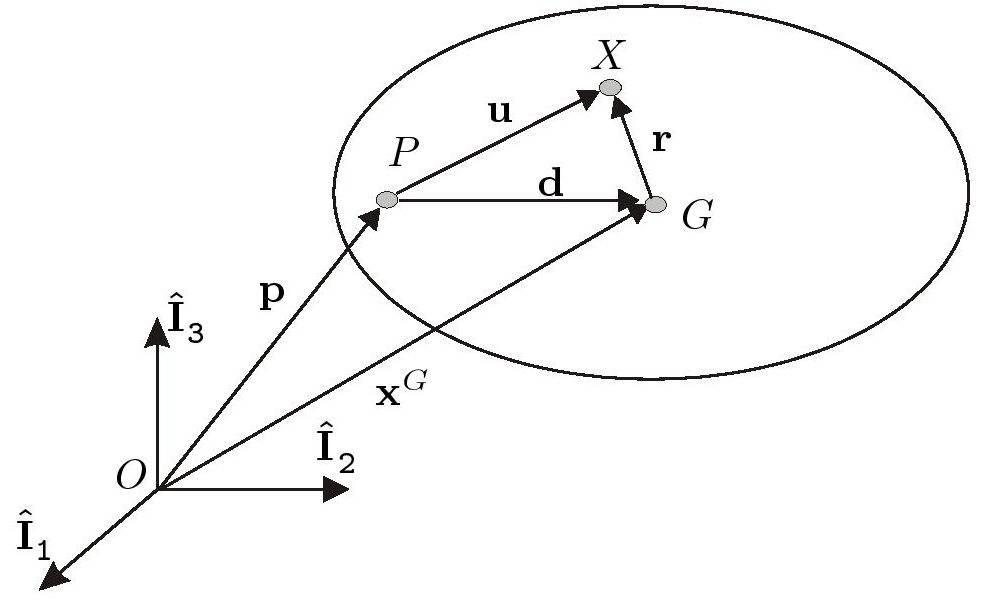
\includegraphics[width=.5\textwidth]{notation.png}
    \caption{\og La patate volante \fg{}}
    \label{fig:patate}
\end{figure}

Tout corps $C$ a un centre de masse unique $G$ définit comme suit
\[ \fv{x}^G = \frac{1}{m} \int_C \fv{x} \dif m \]
$G$ est aussi l'unique point respectant la propriété suivante
\[ \int_C \fv{r} \dif m = \int_C \fvd{r} \dif m = 0 \]
Par la définition d'un corps rigide, les vitesses et accélérations relatives du point $X$
par rapport au repère solidaire du corps $C$ sont nulles :
\[ \fvr{u} = \fvrr{u} = 0 \]

\subsection{Position, vitesse et accélération}
Pour tout \fv{x}, on a
\begin{align*}
    \fv{x} &= \fv{p} + \fv{u} \\
    \fvd{x} &= \fvd{p} + \omegaf\times\fv{u} \\
    \fvdd{x} &= \fvdd{p} + (\omegafd + \omegaf\times\omegaf) \cdot \fv{u}
\end{align*}

\subsection{Quantité de mouvement et moment angulaire}
Soient $\lm$ la quantité de mouvement du corps $C$ et $\am^Q$ le moment angulaire du corps $C$ par rapport au point $Q$.
On a
\begin{align*}
    \lm &= m \fvd{x}^G\\
    \am^O &= \fv{G}^ \times m\fvd{x}^G + \am^G\\
  \am^P &= \int_C \fv{u}\times(\omegaf\times\fv{u}) \dif m = \ine^P \cdot \omegaf
\end{align*}
où $\ine^G \eqdef -\int_C \tilde{\fv{r}}\cdot\tilde{\fv{r}} \dif m$. On l'appelle le \textbf{tenseur d'inertie}.
Il respecte les propriétés suivantes :

\begin{itemize}
    \item ses composantes (exprimées en \si{\kilo\gram\cdot\meter\squared}) sont constantes
        lorsqu'elles sont exprimées dans une base solidaire au corps $C$ ;
    \item il est symétrique ;
    \item il est semi-défini positif ;
    \item
    il existe une base $\base{\uk}$ telle que $\wtr{K}{I}{G}$
    est \textbf{diagonale}, avec $\ine^G = \va{\uk}^T \wtr{K}{I}{G}$; on l'appelle alors la \textbf{matrice principale d'inertie}.
    On appelle les $\uk_i$ les axes principaux d'inertie.
    Les éléments de la diagonale de $\wtr{K}{I}{G}$ sont appelés les moments principaux d'inertie.
    Si un axe principal est un axe de symétrie d'ordre~\footnote{L'ordre d'un axe de symétrie est le nombre d'angle(s) $\theta \in [0; 2\pi[$ tels qu'une rotation de $\theta$ autour de l'axe envoie une forme sur une forme géométriquement identique.
    Par exemple, la diagonale d'un cube est un axe de symétrie d'ordre 3 de celui-ci.} % ça dépend de quel axe on parle, mais pour moi, la diagonale d'un cube est sa grande diagonale, et pas la droite qui joint les centres de deux faces opposées
    $>2$ de $C$, les deux autres axes principaux auront des moments d'inertie égaux ;
  \item
    on peut passer d'un tenseur d'inertie par rapport au point $G$ à ce même tenseur par rapport à un point $P$ avec la formule suivante~\footnote{Si vous vous demandiez pourquoi il y a un signe $-$ dans la formule, alors que logiquement, l'inertie selon $P$ devrait augmenter par rapport à celui selon $G$, sachez que le produit d'une matrice tilde par elle-même a des éléments négatifs sur la diagonale, comme espéré par l'intuition.}
    \[ \ine^P =  \ine^G - m \tilde{\fv{d}}\cdot\tilde{\fv{d}} \]
    Il est primordial que $G$ soit le centre de masse du corps en question pour que cette formule soit correcte !
    C'est la \emph{formule de Steiner} ;
  \item
    si $C = \cup_i \{C_i\}$, alors
    \[ \ine^G = \sum_i \ine_{C^i}^G \]
    Il faut faire attention néanmoins, tous les tenseurs d'inertie doivent
    être exprimés par rapport au même point pour pouvoir être sommés.
    Si ce n'est pas encore le cas, il faut utiliser la formule de
    Steiner pour changer de point de référence ;
  \item lorsqu'il est exprimé par rapport à $G$, on l'appelle le \textbf{tenseur central d'inertie} ;
  \item on peut passer d'un tenseur d'inertie exprimé dans une base $\va{\uj}$ à un
    tenseur d'inertie exprimé dans une base $\va{\uk}$. Si $\va{\uk} = A\va{\uj}$ :
    \[\ine_K = A \ \wrt{J}{\ine} \ A^T\]
\end{itemize}

\paragraph{Interprétation}
Cette interprétation du tenseur d'inertie est inspirée de~\cite{morris2004inertia}.
Le tenseur d'inertie dans l'équation $\amd^G = \tau^G = \ine^G\cdot\omegafd$ a un peu le même
rôle que la masse dans l'équation $\vec{F} = m \vec{a}$, mais pour un mouvement de rotation.
En forme matricielle, l'équation devient :
\[
\begin{pmatrix}
  \tau_x \\
  \tau_y \\
  \tau_z
\end{pmatrix}
=
\begin{pmatrix}
  \ine_{xx} & \ine_{xy} & \ine_{xz} \\
  \ine_{yx} & \ine_{yy} & \ine_{yz} \\
  \ine_{zx} & \ine_{zy} & \ine_{zz}
\end{pmatrix}
\begin{pmatrix}
  \omegafd_x \\
  \omegafd_y \\
  \omegafd_z
\end{pmatrix}
\]

Par exemple, pour un objet tournant autour de l'axe $x$, on a :
\[\tau_x = \ine_{xx} \cdot \omegafd_x\]
Quelques observations à propos de cette équation :
on remarque que plus $\ine_{xx}$ est grand, plus le moment de force
à appliquer autour de l'axe $x$ devra être grand pour faire tourner l'objet.
On remarque aussi que, pour un certain moment de force, si $\ine_{xx} = 0$, on
a une accélération angulaire infinie autour de l'axe $x$, ce qui est impossible.
C'est pour cela que les éléments diagonaux ne sont jamais nuls.

Les éléments non-diagonaux, comme $\ine_{xy}$ par exemple, nous indiquent
\emph{comment l'objet va être accéléré autour de l'axe $y$
lorsque j'applique un moment de force autour de l'axe $x$}.
Cette situation est impossible pour des objets symétriques,
c'est pour cela que les éléments non-diagonaux du tenseur d'inertie d'un objet symétrique
sont nuls.

\subsection{Forces et moments de force}
La somme des moments de force agissant sur un corps $C$ par rapport à un point $Q$ est noté $\st^Q$.

Si la somme des forces est nulle, $\st^Q$ ne dépend pas du choix de $Q$.
On appelle alors $\st^Q$ un \textbf{moment de force pur}\footnote{C'est essentiellement un anglicisme ; en anglais, le moment d'une force est nommé \emph{torque} ou \emph{moment}, un système de forces dont la résultante est nulle mais dont la résultante des moments ne l'est pas est appelé \emph{couple}, \emph{force couple}, ou \emph{pure moment}, et la résultante des moments elle-même est appelé \emph{torque} en mécanique, incitant aux confusions.} et on le note $\pst$.

Si, sur un corps $C$, sont appliquées des forces $\fo^i$ aux points $A^i$ et des purs moments de force $\pst^j$, on a,
\begin{align*}
  \fo &= \sum_i \fo^i\\
  \st^Q &=  \sum_i \vec{QA^i}\times\fo^i + \sum_j \pst^j
\end{align*}

\subsection{Puissance}
Soit $\mathcal{P}$, la puissance correspondante aux forces et aux purs moments de force appliqués au corps $C$.
Elle peut être calculée par la formule suivante
\[ \mathcal{P} = \fo\cdot\fvd{p} + \st^P\cdot\omegaf \]

\subsection{\'Energie cinétique}
Soit $T$, l'énergie cinétique d'un corps $C$.
Elle peut être calculée par la formule suivante
\[ T = \frac{1}{2} \lm \cdot \xgd + \frac{1}{2} \am^G \cdot \omegaf \]
Le premier terme est l'énergie cinétique de translation, tandis que le deuxième
terme est l'énergie cinétique de rotation.

\subsection{Les équations de Newton-Euler}
Comme $\base{\ui}$ est une base inertielle, les 3 lois de Newton s'appliquent
\begin{enumerate}
  \item Si la résultante des forces externes agissant sur un corps $C$ est nulle, alors $\lm$ est constante.
  \item La résultante des forces externes agissant sur un corps $C$ est égale à la dérivée temporelle de sa quantité de mouvement
      \[ \dot{\lm} = m\xgdd = \fo \]
  \item Soit $\fo^{1,2}$, une force appliquée au corps $C^2$ par le corps $C^1$.
    La force de réaction résultante $\fo^{2,1}$ appliquée au corps $C^1$ par le corps $C^2$ est donnée par
    \[ \fo^{2,1} = -\fo^{1,2} \]
\end{enumerate}

Les mêmes lois se transposent très bien pour les moments angulaires et les moments de force.
\begin{enumerate}
  \item Si la résultante des moments de force externes agissant sur un corps $C$ est nulle, alors $\am$ est constant.
  \item La résultante des moments de force externes agissant sur un corps $C$ est égale à la dérivée temporelle de son moment angulaire
    \begin{align*}
      \amd^G &= \st^G\\
             &= \ine^G\cdot\omegafd + \omegaft\cdot\ine^G\cdot\omegaf
    \end{align*}
    La première des deux équations est connue sous le nom d'\emph{équation rotationelle} ou d'\emph{équation d'Euler}. $G$ peut être remplacé par n'importe quel point fixe $O$.

    \paragraph{Remarque}
    Comme le tenseur d'inertie est constant lorsqu'il est exprimé dans une base solidaire
    du corps rigide $C$, on a : $\mathring{\ine}^G = 0$.
  \item Soit $\st^{1,2}$, un moment de force appliqué au corps $C^2$ par le corps $C^1$.
    Le moment de force de réaction résultant $\st^{2,1}$ appliqué au corps $C^1$ par le corps $C^2$ est donné par
    \[ \st^{2,1} = -\st^{1,2} \]
\end{enumerate}

\section{Dynamique de systèmes multicorps}

Supposons qu'on ait $N$ corps rigides avec $c$ contraintes.

\subsection{Coordonnées généralisées}
Si notre problème est en 2D, chaque corps $C_i$ a 3 coordonnées généralisées (sinon, il en a 6, mais supposons qu'on soit en 2D).
\[ \{x_i, y_i, \varphi_i \} \]
Ce qui nous fait $3N$ coordonnées généralisées pour $N$ corps.

\subsection{Contraintes}
Les contraintes sont obtenues le plus souvent de la géométrie du problème et des contraintes de roulement sans glissement.
Nous pouvons alors choisir d'utiliser certaines de nos $c$ contraintes de manière implicite
\footnote{Le plus souvent, on choisit d'utiliser les contraintes de géométrie de manière implicite et celles de roulement sans glissement de manière explicite.},
c'est-à-dire en retirant une coordonnée généralisée apparaissant dans l'équation d'une contrainte.
Posons $c_1$, le nombre de contraintes qu'on utilise de manière implicite.

On aura donc $n \eqdef 3N - c_1$ coordonnées généralisées et $m \eqdef c - c_1$ contraintes explicites.
Notons
\begin{align*}
  q & \eqdef \{q_1, q_2, \ldots, q_n\}\\
  h(q) & \eqdef
      \begin{pmatrix}h_1(q)\\h_2(q)\\\vdots\\h_m(q)\end{pmatrix}\\
  J(q, t) & \eqdef \fpart{h}{q^T}(q, t)\\
          & \eqdef \begin{pmatrix}
            \fpart{h_1}{q_1} & \ldots & \fpart{h_1}{q_n}\\
            \vdots & \ddots & \vdots\\
            \fpart{h_m}{q_1} & \ldots & \fpart{h_m}{q_n}\\
          \end{pmatrix}
\end{align*}
Cette notation nous permet d'écrire que $q$ respecte les contraintes si et seulement si $h(q) = 0$.

\paragraph{Indépendance des contraintes}
Il est ici possible que les contraintes choisies ne soient pas indépendantes.
Il existe un critère assez efficace pour le déterminer
\footnote{Si des contraintes implicites faisaient partie de la dépendance, on peut se convaincre que le raisonnement est correct également.}.

Soit $q$ tel que $h(q) = 0$.
Les contraintes sont indépendantes si et seulement si
\[ \mathrm{rang} (J(q, t)) = m \]

Considérons pour le reste de cette synthèse que les contraintes sont indépendantes.

\subsection{Degré de liberté}
Comme supposé, nos contraintes sont indépendantes.
On a donc $m$ contraintes qui peuvent chacune nous permettre d'exprimer une coordonnée généralisée par rapport aux autres.
Il nous reste donc $n - m$ degrés de liberté.

\subsection{Méthode de Newton-Euler}
Cette méthode permet d'obtenir efficacement les équations du mouvement d'un système multicorps \footnote{On suppose qu'on est en 2D, mais la méthode est aisément extensible en 3D.}. Elle est divisée en 6 étapes :

\paragraph{1. Analyse du système}
On décompose le système en $N$ corps rigides $C_i$, on identifie leurs centres de masse $G^i$
et on leur associe à chacun un repère solidaire $\base{\fv{\hat{X}}^i}$.

\paragraph{2. Choix des coordonnées généralisées et formulation des contraintes}
Par des contraintes implicites liées à la géométrie du système, on réduit nos $3N$ coordonnées à $n$ coordonnées généralisées. À cela s'ajoutent $m$ contraintes explicites indépendantes. On vérifie bien qu'au final on a $n-m$ degrés de liberté.

\paragraph{3. Calculs cinématiques}
À l'aide des coordonnées généralisées, on calcule les moments linéaires $\lm^i$ et angulaires
$\am^i$ de chaque corps et leurs dérivées temporelles. Le calcul du moment angulaire doit se
faire par rapport au centre de masse ou par rapport à un point \textbf{fixe}.

\paragraph{4. Inventaire des forces et moments de force et calcul de leurs résultantes}
Il y a deux types de forces et de moments de force.
\begin{itemize}
  \item Des forces et moments de force qui sont des fonctions connues des positions, orientations et/ou vitesses de certains points du système.
    C'est par exemple la gravité ou la force exercée par une corde attachée au système tout entier.
  \item D'autres forces qui sont introduites pour permettre au système de respecter les contraintes, qu'elles soient implicites ou explicites.
    Par exemple, la force horizontale donnant le moment de force nécessaire à une roue de rouler sur le sol.
    Plus généralement, on peut considérer que chaque contrainte implique une composante d'une force de contrainte.
\end{itemize}

Une fois qu'on a terminé l'inventaire, on calcule la résultante des forces $\fo^i$ et des moments de force $\st^i$ pour chaque corps, par rapport au même point que le moment angulaire.

\paragraph{5. Équations du mouvement}
On écrit les équations de Newton-Euler
\begin{align*}
    \fvd{N}^i &= \fv{F}^i \\
    \amd^i &= \st^i
\end{align*}

ce qui nous donne $3N$ équations scalaires.

\paragraph{6. Solution des équations}
Nous disposons de $3N+m$ équations. Les inconnues sont :
\begin{itemize}
    \item les $n$ coordonnées généralisées ;
    \item \emph{au moins} $3N-n$ composantes de force correspondant aux contraintes implicites ;
    \item $m$ composantes de force correspondant aux contraintes explicites.
\end{itemize}
Ce qui nous fait un total d'au moins $3N+m$ inconnues.
Dans ce cours, le nombre d'inconnues sera toujours égal au nombre d'équations
(système \emph{isostatique}). Autrement, on parle d'un système \emph{hyperstatique}.

Les composantes de force apparaissent toujours linéairement dans les équations ;
il suffira donc de les combiner judicieusement
pour aboutir aux équations différentielles du mouvement qui nous intéressent.
Seulement, on aimerait bien un moyen de trouver la bonne combinaison linéaire de nos équations qui nous donne les équations du mouvement.
C'est là qu'intervient le principe des puissances potentielles.

\section{Principe des puissances potentielles}

L'idée derrière ce principe est de remarquer l'équivalence
\footnote{C'est en fait exactement la même chose que
    $ \alpha\fv{u} + \beta\fv{v} = 0 \ \forall \alpha,\beta
    \Leftrightarrow \fv{u} = \fv{v} = 0 $.}
entre%
\footnote{\og $\land$\fg{} symbolise le \og et\fg{} logique.}
\[
  m\xgdd^i = \fv{F}^i \land
  \amd^i = \st^i
  \quad \text{pour } i = 1, \ldots, N
\]
et
\[
  \sum_{i=1}^N (m\xgdd^i - \fv{F}^i) \cdot \fv{a}^i +
  \sum_{i=1}^N (\amd^i - \st^i) \cdot \fv{b}^i = 0
  \quad \forall \fv{a}^i, \fv{b}^i
\]
Il faut néanmoins que $\fv{a}^i$ et $\fv{b}^i$ aient des unités de telle sorte qu'on puisse sommer les deux termes.
On remarque que donner à $a_j$ les unités de vitesse linéaire et à $b_j$ les unités de vitesse angulaire nous donne des [\si{\watt}] pour les deux termes.
On décide donc de dire que
ce sont des variations potentielles de vitesse et de noter
\begin{align*}
  \fv{a}^i &\eqdef \Delta \xgd^i\\
  \fv{b}^i &\eqdef \Delta \omegaf^i
\end{align*}
Mais attention, ces vecteurs sont juste des coefficients vectoriels arbitraires,
il ne faut donc pas les confondre avec les véritables vitesses $\xgd$ et $\omegaf$ des divers corps.

On définit la variation potentielle de puissance ainsi
\[ \Delta \mathcal{P} \eqdef \sum_{i = 1}^N \left(\fv{F}^i \cdot \Delta \xgd^i + \st^i \cdot \Delta \omegaf^i\right) \]
On peut alors réécrire le principe des puissances potentielles de la manière suivante :
\[\sum_{i=1}^N (m\xgdd^i \cdot \Delta \xgd^i + \amd^i \cdot \Delta \omegaf^i) =
\sum_{i=1}^N (\fv{F}^i \cdot \Delta \xgd^i + \st^i \cdot \Delta \omegaf^i) = \Delta \mathcal{P}\]

Il existe un théorème nous permettant de calculer $\Delta \mathcal{P}$ :

\begin{mytheo}
La contribution d'une force $\fv{F}$ à la variation de puissance due aux changements
virtuels de $\Delta \xgd^i$ et $\Delta \omegaf^i$ est égal au produit de cette force avec
le changement virtuel de vitesse de son point d'application.
\begin{equation}
\Delta \mathcal{P}_{\fv{F}^A} = \fv{F}^A \cdot \Delta \xgd^A
\label{eq:ppp_delta}
  \end{equation}
\end{mytheo}

Ce théorème permet de calculer la variation de puissance plus facilement (particulièrement dans le
cas où la vitesse virtuelle du point d'application de la force est nulle).

\subsection{Choix des variations potentielles de vitesse}
\subsubsection{Choix compatibles}
L'idée, c'est qu'on aimerait choisir des $\Delta \xgd^i$ et des $\Delta \omegaf^i$ tels que les forces de contrainte disparaissent de l'équation.
Pour nous aider, il y a un théorème très fort qui dit
\begin{mytheo}
    Si des variations potentielles de vitesse $\Delta \xgd^i$ et des
    $\Delta \omegaf^i$ sont compatibles avec une contrainte,
    sa force de contrainte correspondante n'aura aucune influence
    sur $\Delta \mathcal{P}$,
    elle disparaitra de l'équation des puissances potentielles.
\end{mytheo}

Il nous suffit donc de trouver des variations potentielles de vitesse compatibles avec toutes les contraintes.

\paragraph{Remarque}
Si jamais on a, par exemple, un corps qui glisse sur le sol et qu'on décide de considérer ses frottements,
on ne peut pas dire qu'ils disparaitront quand les variations potentielles de vitesses seront compatibles avec la contrainte relative à la force normale.
Comme la force de frottement est proportionnelle à la force normale, il vaudra mieux dans ce cas ne pas éliminer cette dernière de l'équation mais prendre deux choix différents de variations potentielles de vitesse pour avoir 2 équations :
une pour les équations du mouvement et une pour se débarrasser de la force normale.
%TODO expliquer plus en détail comment obtenir la valeur d'une force, avec la procédure de "cassage" de mécanisme.

\subsubsection{Choix non-compatibles}
Il arrive parfois que l'on veuille calculer une force de contrainte spécifique. On peut alors
faire un choix de vitesses potentielles non-compatibles avec les contraintes afin de les
faire apparaître dans l'équation.

\subsection{Calcul de variations potentielles de vitesse compatibles}
Pour cela, il faut choisir des $\dqp$ compatibles, c'est à dire tels que
\[ J(q, t) \dqp = 0 \]
Ensuite,
comme on sait que $\xgd^i$ et $\omegaf^i$
sont linéairement dépendants des $\qp_\alpha$%
\footnote{Preuve à la p.~47 du syllabus.}%
, on a
\begin{align*}
  \Delta \xgd^i &= \sum_{\alpha = 1}^n \fpart{\xgd^i}{\qp_\alpha} \dqp_\alpha\\
  \Delta \omegaf^i &= \sum_{\alpha = 1}^n \fpart{\omegaf^i}{\qp_\alpha} \dqp_\alpha
\end{align*}

\paragraph{Exemple}
Si
\begin{align*}
  q &= \{q_1, q_2\}\\
h(q) &= \begin{pmatrix}q_1 - 2q_2\end{pmatrix}\\
  \xgd &= 2\qp_1 \ui_1 + (q_1 + 3\qp_2) \ui_2
\end{align*}
On a $J(q, t) = \begin{pmatrix}1 & -2\end{pmatrix}$.
Les variations potentielles de vitesse sont donc de la forme $\dqp = \{2\Delta v_1, \Delta v_1\}$.
\begin{align*}
  \Delta \xgd^i &= 2 \dqp_1 \ui_1 + 3 \dqp_2 \ui_2\\
                &= (4\ui_1 + 3\ui_2) \Delta v_1
\end{align*}

% The contribution of a force F to the virtual power change due to virtual velocity changes dx and dw is equal to the dot product of this force with the virtual velocity change of its application point resulting from dx and dw. p.73

\subsection{Calcul des équations du mouvement}
Nous avons donc exprimé nos vitesses potentielles $\Delta q_\alpha$ par rapport à $n - m$ paramètres $\Delta v_\beta$ pour que les coordonnées généralisées respectent les contraintes.
Nous pouvons maintenant résoudre notre équation des puissances potentielles.
Comme nous respectons les contraintes, toutes les forces de contrainte vont disparaitre de l'expression.
Dès lors, pour simplifier vos calculs, vous pouvez ne pas les prendre en compte (si vous n'êtes pas sûr, mettez-les, vous verrez, elles vont se simplifier).
Vous terminez donc avec
\[ \sum_{\beta = 1}^{n - m} c_\beta \Delta v_\beta = 0 \]
Comme les $\Delta v_\beta$ sont des paramètres, ils peuvent avoir la valeur que vous désirez
(comme par exemple, tous 0 sauf un).
On a donc
\[ c_\beta = 0 \quad \text{pour }\beta = 1, 2, \ldots, n-m \]
Ce qui, avec les $m$ contraintes, constitue un système de $n$ équations différentielles pour nos $n$ inconnues.

\section{Méthode des multiplicateurs de Lagrange}

\subsection{Explication de la méthode des multiplicateurs de Lagrange}
Comme vu précédemment, les $\Delta \xgd^i$ et les $\Delta \omegaf^i$ dépendent linéairement des $\dqp_\alpha$.
Du coup, si on calcule la formule des puissances potentielles sans les forces de contrainte, il existera des coefficients $Q'_\alpha$
\footnote{On les appelle les $Q'_\alpha$ et non les $Q_\alpha$ pour suivre la notation du livre où les $Q_\alpha$ sont déjà définis.}
tels que la formule vaudra
\[ \sum_{\alpha = 1}^n Q'_\alpha \dqp_\alpha =
\begin{pmatrix}Q'_1 & Q'_2 & \ldots & Q'_n\end{pmatrix}\begin{pmatrix}\dqp_1\\\dqp_2\\\ldots\\\dqp_n\end{pmatrix}
= (Q')^T \dqp \]
Seulement, on sait que si $\dqp$ respecte les contraintes, alors, le fait d'avoir ignoré les forces de contrainte n'a pas d'influence et la formule des puissances potentielles est correcte et donc $(Q')^T \dqp = 0$.
Autrement dit,
\[ J(q, t) \dqp = 0 \Rightarrow (Q')^T \dqp = 0 \]
Vectoriellement parlant, si $\dqp$ est orthogonal aux lignes de $J(q, t)$, alors $\dqp$ est orthogonal à $Q'$.
Un peu d'algèbre détaillée dans l'annexe~\ref{ann:orthogonal}, nous indique que ça signifie que $Q'$ est une combinaison linéaire des lignes de $J(q, t)$.
C'est à dire qu'il existe des $\lambda_j$ tels que
\begin{align*}
  Q' &= \sum_{j = 1}^m l_j^T \lambda_j\\
Q' &= \begin{pmatrix}l_1^T&l_2^T&\ldots&l_m^T\end{pmatrix} \begin{pmatrix}\lambda_1\\\lambda_2\\\vdots\\\lambda_m\end{pmatrix}\\
  Q' &= J^T(q, t) \lambda
\end{align*}
Ce qui nous donne $n$ équations avec $m$ variables supplémentaires $\lambda_j$.
En se débarrassant des $\lambda_j$, on perd $m$ équations et on se retrouve avec $n - m$ équations qui, avec les $m$ contraintes, font $n$ équations différentielles.
On était arrivé à la même chose avec la méthode des puissances potentielles mais, cette fois-ci, nous les avons obtenues sans utiliser d'astuce algébrique.

\subsection{Application de la méthode des multiplicateurs de Lagrange}

\subsubsection{Calcul des $Q'_\alpha$}
On sait qu'en calculant la formule des puissances potentielles en ignorant les forces de contrainte,
on trouve $\sum_{\alpha = 1}^n Q'_\alpha \dqp_\alpha$.
De là, on peut voir deux manières d'isoler les $Q'_\alpha$.
\begin{enumerate}
  \item On prend $\dqp = \{\dqp_1, \dqp_2, \ldots, \dqp_n\}$, on exprime les $\Delta \xgd^i$ et les $\Delta \omegaf^i$ en fonction,
    et on met les $\dqp_\alpha$ en évidence dans la formule des puissances potentielles (sans prendre en compte les forces de contraintes) pour faire apparaitre les $Q'_\alpha$.
  \item On prend $n$ choix de $\dqp$, $\{\dqp_1, 0, \ldots, 0\}, \{0, \dqp_2, 0, \ldots, 0\}, \ldots, \{0, \ldots, 0, \dqp_n\}$.
    Pour chacun, on exprime les $\Delta \xgd^i$ et les $\Delta \omegaf^i$ en fonction de l'unique $\dqp_\alpha$ non nul.
    On met alors $\dqp_\alpha$ en évidence dans la formule des puissances potentielles (sans prendre en compte les forces de contrainte) pour faire apparaître $Q'_\alpha$.
\end{enumerate}

\subsubsection{Utilisation des $Q'_\alpha$}
On écrit alors
\[ Q' = J^T(q, t) \lambda \]
Ce qui nous fait $n$ équations.
On en utilise $m$ pour faire disparaître les $\lambda$.
On a alors, avec les $m$ contraintes, $n$ équations différentielles décrivant le mouvement.


\part{Statique}

Dire qu'un corps est statique ou à l'équilibre équivaut à dire que
\begin{align*}
  \fv{F} &= 0\\
  \st^Q &= 0
\end{align*}
On remarque que dans le cas d'un corps à l'équilibre, $\st^Q$ ne dépend pas du point $Q$.
En effet, $\st^{Q_2} = \st^{Q_1} + \vec{Q_2Q_1} \times \fv{F} = \st^{Q_1}$.

\paragraph{Remarque}
Les problèmes analysés sont des problèmes plans, les couples seront donc toujours orthogonaux aux forces.
$\fv{F} = 0$ ne donnera que deux équations scalaires non triviales et $\st^Q$ n'en donnera qu'une.

\section{Liaisons et appuis plans usuels}
Les principaux types de liaisons dans le plan se distinguent par le nombre et le type de contraintes qu'elles imposent, et donc par les degrés de libertés restantes. Chaque contrainte donnent lieu à une inconnue, qui est la valeur de la force ou du moment imposant cette contrainte. L'objectif est de déterminer ces inconnues.
% See package TikZ-mec.
\subsection{Appui fixe}
Symbolisé par un triangle avec un sommet touchant le corps.
Il produit deux forces, une horizontale et une verticale. Il a le même effet qu'une articulation rotoïde, et ne permet qu'une rotation% C'est bien de l'appui qu'on parle?

\subsection{Appui simple (ou appui à rouleau)}
Symbolisé par un cercle touchant le corps.
Il produit une force, perpendiculaire à la tangente du cercle au point de contact, et laisse un degré de liberté en plus que l'appui fixe.

\subsection{Glissière (sans frottement)}
Elle produit une force perpendiculaire à la glissière et un couple rentrant dans le plan, n'autorisant qu'une translation dans une direction précise.

\subsection{Encastrement plan}
Il produit une force perpendiculaire à l'encastrement, une force parallèle et un couple rentrant dans le plan.

\section{Efforts internes}
On peut s'intéresser aux efforts internes d'un corps, c'est à dire les forces exercées à l'intérieur d'une coupe théorique du corps.
Pour cela, il suffit d'imaginer de désolidariser le corps à l'endroit de la coupe.
\begin{itemize}
  \item Le moment fléchissant $M_f$ est positif dans le sens d'une compression des fibres supérieures et d'un étirement des fibres inférieures (concavité vers le haut) ;
  \item L'effort tranchant $T$ est positif s'il induit une rotation horaire de la matière à laquelle il est associé ;
  \item L'effort normal $N$ est positif en traction.
\end{itemize}

On calcule donc leur valeur pour qu'on ait l'équilibre d'un côté ou l'autre du corps désolidarisé (on devrait avoir la même valeur des deux côtés vu que les forces et les couples sont définis dans un sens opposé si on prend la coupe à gauche ou à droite).

\paragraph{Remarque}
La définition du sens des vecteurs est juste une convention, il se peut que vous trouviez une valeur négative pour vos forces.
Mais ce n'est pas une raison pour ne pas la respecter.

\subsection{Diagrammes d'efforts internes}
Il est parfois demandé de dessiner des diagrammes d'efforts internes. Ce sont des diagrammes qui représentent
la valeur d'un effort interne en fonction de la position $x$ de la \og coupure\fg{}. Par convention, ces diagrammes
sont dessinés avec l'ordonnée positive vers le bas.

On remarque également que :
\[T(x) = \fdif{M(x)}{x}\]

\section{Résolution classique dans le plan}
Un problème de statique dans le plan peut se résoudre selon les étapes suivantes :

\begin{enumerate}
  \item On dessine dans un premiers temps les couples et forces de réaction aux différentes liaisons et appuis ;
  \item On vérifie ensuite que le nombre d'inconnues n'est pas $> 3$, auquel cas nous serions face à un système \emph{hyperstatique} ;
  \item On écrit ensuite les équations :
    \begin{align*}
      \sum \fv{F}_x &= 0 \\
      \sum \fv{F}_y &= 0 \\
      \sum \st^Q    &= 0
    \end{align*}
  \item Si demandé, on dessine les différents diagrammes d'efforts internes.
\end{enumerate}

\annexe
\section{Preuve de l'appartenance de $Q'$ à l'espace des lignes de $J(q, t)$}
\label{ann:orthogonal}
\begin{proof}
  Soient $l_1^T, l_2^T, \ldots, l_m^T$ les lignes de $J(q, t)$ et $V$ le sous espace vectoriel de $\mathbb{R}^N$ qu'elles engendrent.
  Comme on suppose que les contraintes sont indépendantes, $\mathrm{rang}(J(q, t)) = m$, et donc les $l_j^T$ sont une base de $V$.
  Prenons la projection $v \in V$ de $Q'$ dans $E$, on sait qu'il existe $w \in V^\perp$ tels que
  \[ Q' = v + w \]
  On sait que $v^Tw = 0$ donc comme les $l_j^t$ sont une base de V, $J^T(q, t)w = 0$.
  Dès lors, $Q'^T w = 0$.
  Par conséquent, $(v + w)^T w = 0$, c'est à dire $w^T w = 0$.
  Comme le produit scalaire est défini positif, ça signifie que $w = 0$ et donc $Q' = v$ et $Q' \in V$.
\end{proof}

\section{Masse ponctuelle et vitesse angulaire}
On pourrait se demander ce que vaut $\omegaf$ pour un corps modélisé par une masse ponctuelle.
En effet, si un corps est sans dimension, comment peut on déterminer $\omegaf$ ?

Pour voir clair ici, il faut se rappeler que $\omegaf$ est lié à deux bases, pas à un corps.
Lorsqu'on lie $\omegaf$ à un corps, on veut implicitement parler de $\omegaf^{JI}$ où $\va{\uj}$ est la base cure-dent du corps.
Mais que vaut la base cure-dent d'un corps sans dimension ?

En fait, la question est plutôt, a-t-on besoin de $\omegaf$ ?
\begin{itemize}
  \item Pour calculer $\xgd$,
    il suffit de regarder dans quelle base est exprimé $\xg$.
    Si cette base est $\base{\uj}$, alors on prend $\omegaf^{JI}$;
  \item Pour calculer $\am^G$ et $\lm^G$, comme le corps n'a pas de dimension, $\ine^G = 0$\footnote{
    Attention : bien qu'une masse ponctuelle n'aie pas d'inertie par rapport à son \og centre de masse\fg{}, elle a quand même
    une inertie par rapport aux points qui l'entourent. On peut la calculer en utilisant Steiner.} et $\vec{GA^i} = 0$
    pour tout $\fo^i$, donc
    $\am^G = 0 = \amd^G$ et $\lm^G = 0$;
  \item Pour calculer $(\amd^G - \lm^G) \cdot \Delta \omegaf$, on a, pour les même raison que le point précédent,
    $\amd^G - \lm^G = 0 - 0 = 0$, donc $(\amd^G - \lm^G) \cdot \Delta \omegaf = 0$.
\end{itemize}

\biblio

\end{document}
